\subsection{Resultados De Escenario Experimental A}

El objetivo de las pruebas realizadas en el presente escenario experimental, era validar que, los procesos implementados, efectivamente realizaran la adaptación de las aplicaciones desde un estado de completa falla, en donde ninguno de los datos necesarios estuviera presente.

Siguiendo los pasos definidos en la sección \ref{sec:EscenarioExperimentalA}, se realizó el despliegue de los servicios base de Smart Campus UIS, al igual que \textit{Bran} y \textit{DoThing}. Como se presenta en la figura \ref{fig:LookerStart}, se registró el estado de referencia al agregador tras validarlo usando \textit{Lexical}, y se fijaron las directivas a usar para la adaptación de la arquitectura.

\begin{figure}[ht]
    \centering
    \caption{Aplicación y directivas registradas en Bran}
    \label{fig:BranStart}
    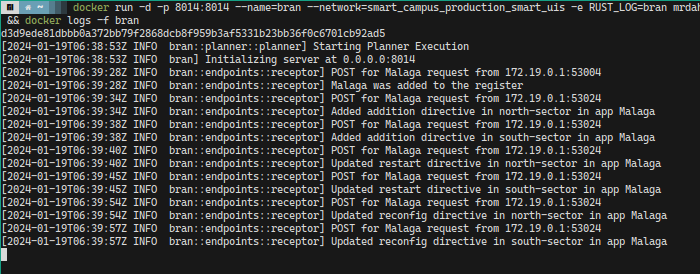
\includegraphics[width=0.9\linewidth]{images/BranStart.png}
    \vspace{-4mm}
\end{figure}

Una vez se inició el servicio \textit{Looker}, como se ve en la figura \ref{fig:LookerStart}, este empezó a evaluar el estado de la aplicación; que al no tener ningún tipo de reporte de algún componente, entró directamente en estado de falla. 

\begin{figure}[ht]
    \centering
    \caption{Looker evalúa el estado de la aplicación}
    \label{fig:LookerStart}
    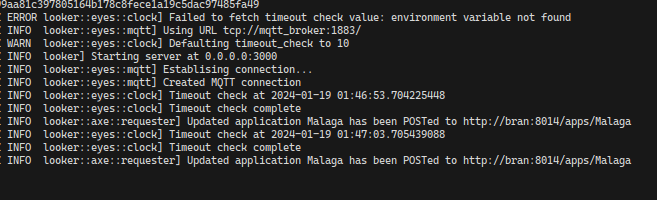
\includegraphics[width=0.9\linewidth]{images/LookerStart.png}
    \vspace{-4mm}
\end{figure}

El estado observado, se reportó a \textit{Bran}, el cual, realizó el recorrido para identificar los puntos de falla de la aplicación. Como se observa en la figura \ref{fig:BranPlan}, como era de esperar, los tres requerimientos definidos en cada una de las locaciones estaba en estado de falla. Al no haber componentes reportando datos, como era de esperarse, se definieron acciones \textit{Addition} para todos los componentes de la aplicación. 

\begin{figure}[ht]
    \centering
    \caption{Bran identifica los problemas y establece las acciones}
    \label{fig:BranPlan}
    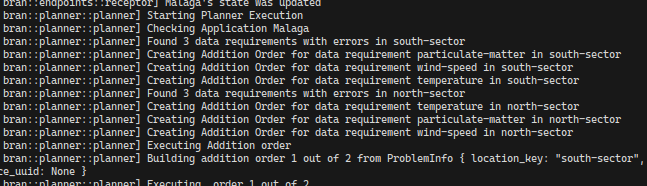
\includegraphics[width=0.9\linewidth]{images/BranPlanning.png}
    \vspace{-4mm}
\end{figure}

A partir de las acciones, se crearon las órdenes para ejecución usando las directivas como base. Como se puede ver en la figura \ref{fig:DoThingDoing}, cada una de estas se envió a \textit{DoThing}, el cual realizó el procesamiento requerido para la construcción y arranque de los contenedores. El resultado de este procesamiento se puede ver en la figura \ref{fig:ContainerState}

\begin{figure}[ht]
    \centering
    \caption{DoThing ejecuta las acciones establecidas por Bran }
    \label{fig:DoThingDoing}
    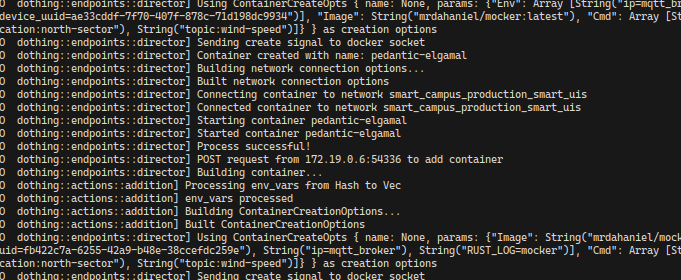
\includegraphics[width=0.9\linewidth]{images/DoThingDoing.png}
    \vspace{-4mm}
\end{figure}

\begin{figure}[ht]
    \centering
    \caption{Contenedores creados por DoThing en respuesta a las órdenes recibidas}
    \label{fig:ContainerState}
    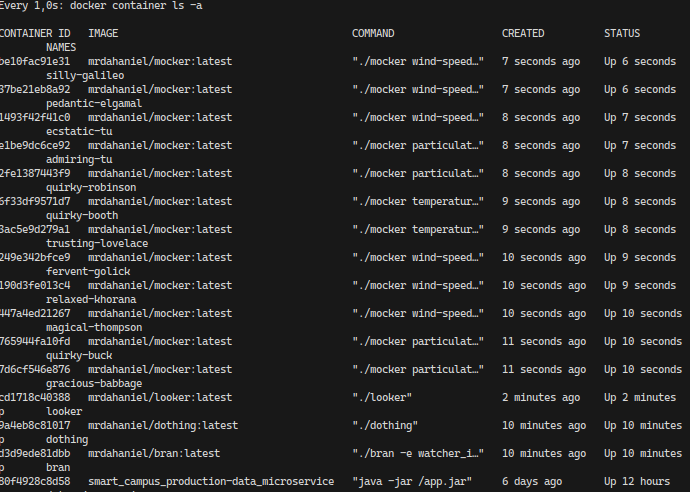
\includegraphics[width=1\linewidth]{images/ContainerLaunching.png}
    \vspace{-4mm}
\end{figure}

En total, se crearon 12 contenedores, que corresponden a los 12 componentes requeridos para el desarrollo de la aplicación. Cada uno de ellos configurado para suplir las necesidades de operación establecidas en el estado de referencia. Estos despliegues, como era de esperarse, fueron detectado por \textit{looker}, el cual realizó el nuevas valoraciones del estado. 

Los valores por defecto de los servicios usados para estas pruebas es un intervalo de tiempo entre mensajes de un minuto. Este valor por defecto, aunque para los requerimientos de datos cuyos \textit{timeout}, sean superiores, supliría las necesidades de la aplicación. Sin embargo, en el marco de esta simulación, esta frecuencia de reportes no es suficiente para cumplir con el estado de referencia de los requerimiento de temperatura de las locaciones.

Como consecuencia, el estado de la aplicación regresó a estado \textit{Fault}, y \textit{Bran}, al detectar los problemas, emitió las acciones tipo \textit{Restart} con el fin de traer los contenedores a un estado válido. Esto se puede ver en la figura \ref{fig:BranPlan2}.

\begin{figure}[ht]
    \centering
    \caption{Bran identifica otros problemas en la aplicación}
    \label{fig:BranPlan2}
    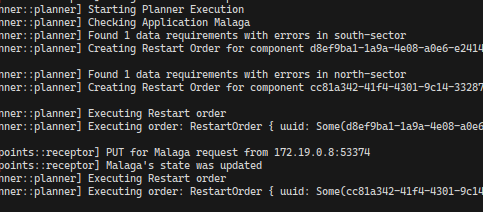
\includegraphics[width=0.9\linewidth]{images/BranRestarting.png}
    \vspace{-4mm}
\end{figure}

Este intento de reiniciar los servicios, como era de esperarse, no fue realmente efectiva debido a que la falla se debe a un problema en la configuración del servicio. Siendo así, la aplicación se mantuvo en estado de falla. Se esperaba que, ambos componentes encargados de la temperatura, al ya haber descartado el reinicio como un mecanismo efectivo para esta situación, fueran sometidos a una acción de reconfiguración, sin embargo, como se observa en la figura \ref{fig:BranPlan3}, en ese instante, sólo el componente de \texttt{north-sector} fue afectado.

\begin{figure}[ht]
    \centering
    \caption{Bran establece acciones de reconfiguración para adaptar la aplicación}
    \label{fig:BranPlan3}
    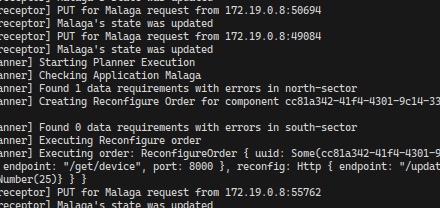
\includegraphics[width=0.9\linewidth]{images/BranReconfiguring.png}
    \vspace{-4mm}
\end{figure}

Esta reconfiguración fue ejecutada por \textit{DoThing}, y tomó efecto, alterando el valor por defecto entre mensajes, pasando de un reporte cada minuto, a uno cada 25 segundos\footnote{Según lo definido en las directivas presentes en el apéndice \ref{ape:DirectivesA}}. Con el nuevo valor, los componentes de temperatura, empezaban a reportar con mayor frecuencia, cumpliendo con las expectativas.

Poco tiempo después, el componente de temperatura de \texttt{south-sector}, reportó el estado de falla, por lo se ejecutó la misma acción de reconfiguración que con el componente de la otra locación, llevando el estado de la aplicación a \textit{Coherent}.

A partir de esta simulación, se pudo validar que el proceso implementado, tiene la capacidad de realizar la adaptación desde el peor escenario, hacia un esto de coherencia con la aplicación declarada inicialmente. Todas las acciones definidas por \textit{Bran}, permitieron modificar el estado de manera positiva.

Sin embargo, se identificaron algunas limitaciones de esta implementación. Como se observa en la figura \ref{fig:BranPlan3}, se muestra que \texttt{south-sector} no presenta problemas en sus requerimientos, cuando, debido a su configuración, debía estar en estado de falla. 

Esto se debe a un \textit{quirk} de la implementación realizada. Al manejar los procesos cada cierto intervalo de tiempo, es posible que un componente se encuentren en estado de falla, pero alcance a pasar a coherente justo antes de la evaluación de las acciones a tomar. Eventualmente, el componente fallaría en reportar antes de una una de las evaluaciones desencadenando en una acción, como fue el caso con la tardía reconfiguración del componente de \texttt{south-sector}. 